\documentclass[varwidth=true, border=2pt]{standalone}

\usepackage{pgfplots}
\usepackage{tikz}

\usetikzlibrary{calc,patterns,angles,quotes}

\begin{document}

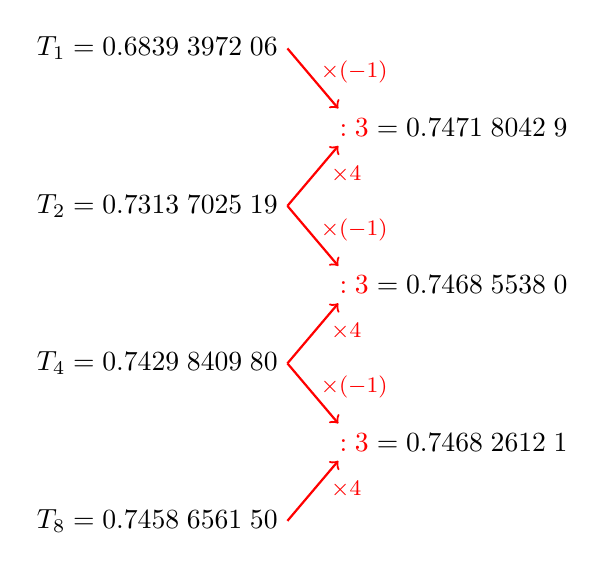
\begin{tikzpicture}



	\node (T1) at (1,7) {$T_1 = 0.6839 \; 3972 \; 06$};
	\node (T2) at (1,5) {$T_2 = 0.7313 \;7025 \; 19$};
	\node (T4) at (1,3) {$T_4 = 0.7429 \; 8409 \; 80$};
	\node (T8) at (1,1) {$T_8 = 0.7458 \; 6561 \; 50$}; %Some uncertainty about last 2 digits.  Maybe recalculate in MATLAB
	\node (A1)[red] at (3.5, 6){$:3$};
	\node (A2)[red] at (3.5, 4){$:3$};
	\node (A3)[red] at (3.5, 2){$:3$};
	
	\node (B1) at (5,6){$= 0.7471\;8042\;9$};
	\node (B2) at (5,4){$= 0.7468\;5538\;0$};
	\node (B3) at (5,2){$= 0.7468\;2612\;1$};
	
%	\node (D1)[red] at (7, 5){$:15$};
%	\node (D2)[red] at (7, 3){$:15$};
	
%	\node (E1) at (8.5,5){$= 0.7468\;3371\;0$};
%	\node (E1) at (8.5,3){$= 0.7468\;2417\;0$};
	
%	\node (F1)[red] at (11, 4){$:63$};

	\draw [->, thick,red] (T1.east) to (A1);
	\draw [->, thick,red] (T2.east) to (A1);
	\draw [->, thick,red] (T2.east) to (A2);
	\draw [->, thick,red] (T4.east) to (A2);
	\draw [->, thick,red] (T4.east) to (A3);
	\draw [->, thick,red] (T8.east) to (A3);
%	\draw [->, thick,red] (B1.east) to (D1);
%	\draw [->, thick,red] (B2.east) to (D1);
%	\draw [->, thick,red] (B2.east) to (D2);
%	\draw [->, thick,red] (B3.east) to (D2);

	\node (A1a)[red] at (3.5,6.7){\footnotesize{$\times (-1)$}};
	\node (A1b)[red] at (3.4,5.4){\footnotesize{$\times 4$}};
	\node (A2a)[red] at (3.5,4.7){\footnotesize{$\times (-1)$}};	
	\node (A2b)[red] at (3.4,3.4){\footnotesize{$\times 4$}};
	\node (A3a)[red] at (3.5,2.7){\footnotesize{$\times (-1)$}};	
	\node (A3b)[red] at (3.4,1.4){\footnotesize{$\times 4$}};
%	\node (D1a)[red] at (7.8,5.7){\footnotesize{$\times (-1)$}};
%	\node (D1b)[red] at (7.7,4.4){\footnotesize{$\times 16$}};
%	\node (D2a)[red] at (7.8,3.7){\footnotesize{$\times (-1)$}};
%	\node (D2b)[red] at (7.7,2.4){\footnotesize{$\times 16$}};	
	
\normalsize
	
\end{tikzpicture}
\end{document}